\documentclass[a4paper, 12pts]{amsart}

\usepackage[utf8]{inputenc}
\usepackage{listings}
\usepackage{datetime}
\usepackage{tikz}
\usetikzlibrary{arrows}

\newdateformat{monthyeardate}{
  \monthname[\THEMONTH], \THEYEAR}

\title{Different to the Minimizing Function on Neural Networks}
\author{Ortega Andrés, Fonseca Diego, Calad Juan\\
  \monthyeardate{\today}}

\begin{document}
\maketitle
\tableofcontents
\section{Basics on Neural Networks}
A neural network can be viewed as a directed graph in which each vertex serves
as a ``neuron'' and have an associated output value for how active it is.
For the first layer of neurons, their output values are simply input given to
the network. In the case of other neurons it will calculated taking into
account the activation values of all neurons connected to it. The output or
``return'' value of the neural network will be how active are all the neurons
that have no connections, or the ones belonging to the output layer. It is
common to have a set of intermediate neurons between the input and output layer
in order to give the network the capability of more complex tasks.

\begin{figure}[!h]
  \centering
  \def\layersep{2.5cm}

  \begin{tikzpicture}[shorten >=1pt,->,draw=black!50, node distance=\layersep]
    \tikzstyle{every pin edge}=[<-,shorten <=1pt]
    \tikzstyle{neuron}=[circle,draw,minimum size=17pt,inner sep=0pt]
    \tikzstyle{annot} = [text width=4em, text centered]

    % Draw the input layer nodes
    \foreach \y in {1,...,4}
    % This is the same as writing \foreach \name / \y in {1/1,2/2,3/3,4/4}
    \node[neuron, pin=left:$x_\y$] (I-\y) at (0,-\y) {};

    % Draw the hidden layer nodes
    \foreach \y in {1,...,5}
    \path[yshift=0.5cm]
    node[neuron] (H-\y) at (\layersep,-\y cm) {};

    % Draw the output layer node
    \node[neuron,pin={[pin edge={->}]right:Output}, right of=H-3] (O) {};

    % Connect every node in the input layer with every node in the
    % hidden layer.
    \foreach \source in {1,...,4}
    \foreach \dest in {1,...,5}
    \path (I-\source) edge (H-\dest);

    % Connect every node in the hidden layer with the output layer
    \foreach \source in {1,...,5}
    \path (H-\source) edge (O);

    % Annotate the layers
    \node[annot,above of=H-1, node distance=1cm] (hl) {Hidden layer};
    \node[annot,left of=hl] {Input layer};
    \node[annot,right of=hl] {Output layer};
  \end{tikzpicture}
  \caption{Example of a neural network}
\end{figure}

The value of each neuron will take will be a function of a the weighted sum
of all neurons connected to it plus a bias. If we take $W_n$ as a matrix with
the weights of each neuron from layer $n-1$ to $n$, $b_n$ the associated bias
of each neuron in layer $n$ and $a_n$ the value of each neuron in layer $n$
then we would have:
\[a_n=f(Wa_{n-1}+b)\]

It is common for the sigmoid function ($\sigma(x)=\frac{1}{1+e^{-x}}$)
to be used as activation function for having certain characteristics.
These characteristics include being monotonic, differentiable, having domain
over all $\mathbb{R}$ and having range $(0,1)$. For this motive in the current
document the sigmoid function will also be used as the activation function.

Defining
\[\sigma\left(
  \begin{bmatrix}
    a_1\\
    a_2\\
    \vdots\\
    a_n
  \end{bmatrix}
  \right) =
  \begin{bmatrix}
    \sigma(a_1)\\
    \sigma(a_2)\\
    \vdots\\
    \sigma(a_n)
  \end{bmatrix}
\]
We would end up with
\[a_n=\sigma(Wa_{n-1}+b)\]


\begin{figure}[!h]
  \centering
  \def\layersep{2.5cm}

  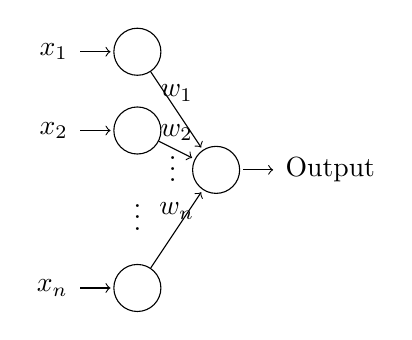
\begin{tikzpicture}[shorten >=1pt,->, node distance=\layersep]
    \tikzstyle{every pin edge}=[<-,shorten <=1pt]
    \tikzstyle{neuron}=[circle,draw,minimum size=17pt,text height=.5ex,
    inner sep=1pt]

    \node[neuron, pin=left:$x_1$] (I-1) at (0,-1) {};
    \node[neuron, pin=left:$x_2$] (I-2) at (0,-2) {};
    \node (D) at (0,-3) {$\vdots$};
    \node[neuron, pin=left:$x_n$] (I-n) at (0,-4) {};
    
    \node[neuron,pin={[pin edge={->}]right:Output}] (O) at (\layersep,-2.5) {};

    \path (I-1) edge node [above] {$w_1$} (O)
          (I-2) edge node [above] {$w_2$} (O)
          (D)   edge [draw=none] node [above] {$\vdots$} (O)
          (I-n) edge node [above] {$w_n$} (O);

  \end{tikzpicture}
  \caption{Weights in a neural network}
\end{figure}
\section{Training the Network}
To train the network a initial test data set, composed by the input and the expected output, is used. The objective is to compare the expected output and the network's output, using the error function as proposed:

\[E(\hat{y}, y) = \frac{1}{2n}\sum_{i=1}^{n} (y_i-\hat{y_i})^2\]


With these results we can modify each weight and bias. This will result in the network giving an output closer to the expected one. After many tests the change in weights and biases will be determined by using the partial derivatives of the cost function in respect to the weights and in respect to the biases, resulting in the gradient which we seek to minimize in order to get the best results:

\[\nabla C = \frac{\partial C}{\partial W}\]

To get the next position we desire to advance to we use these equations:

\[ w'_k = w_k - \eta\frac{\partial C}{\partial w_k}\]


\[b'_k = b_k - \eta\frac{\partial C}{\partial b_k}\]

Where $w_k$ are the network's weight, $b_k$ are the network's biases, and $\eta$ is the learning factor which determines how far we will advance.


\[
  \begin{bmatrix}
    z_{1}^{l}\\
    z_{2}^{l}\\
    \vdots\\
    z_{n}^{l}
  \end{bmatrix}
   =
   \begin{bmatrix}
    w_{11} & w_{12} & w_{13} & \dots  & w_{1p} \\
    w_{21} & w_{22} & w_{23} & \dots  & w_{2p} \\
    \vdots & \vdots & \vdots & \ddots & \vdots \\
    w_{n1} & w_{n2} & w_{n3} & \dots  & w_{np}
\end{bmatrix}
   \begin{bmatrix}
    a_{1}^{l-1}\\
    a_{2}^{l-1}\\
    \vdots\\
    a_{p}^{l-1}
  \end{bmatrix}
  +
  \begin{bmatrix}
    b_{1}^{l}\\
    b_{2}^{l}\\
    \vdots\\
    b_{n}^{l}
  \end{bmatrix}
\]

\[
  \begin{bmatrix}
    a_{1}^{l}\\
    a_{2}^{l}\\
    \vdots\\
    a_{n}^{l}
  \end{bmatrix}
   =
  \begin{bmatrix}
    \sigma(z_{1}^{l})\\
    \sigma(z_{2}^{l})\\
    \vdots\\
    \sigma(z_{n}^{l})
  \end{bmatrix}
\]
\\
\\

\begin{figure}[!h]
  \centering
  \def\layersep{2.5cm}

  \begin{tikzpicture}[shorten >=1pt,->,draw=black!50, node distance=\layersep]
    \tikzstyle{every pin edge}=[<-,shorten <=1pt]
    \tikzstyle{neuron}=[circle,draw,minimum size=17pt,inner sep=0pt]
    \tikzstyle{annot} = [text width=4em, text centered]

    % Draw the input layer nodes
    \foreach \y in {1,...,4}
    % This is the same as writing \foreach \name / \y in {1/1,2/2,3/3,4/4}
    \node[neuron, pin=left:$x_\y$] (I-\y) at (0,-\y) {};

    % Draw the hidden layer nodes
    \foreach \y in {1,...,5}
    \path[yshift=0.5cm]
    node[neuron] (H-\y) at (\layersep,-\y cm) {};

    % Draw the output layer node
    \foreach \y in {1,...,3}
    \path[yshift=-0.5cm]
    node[neuron, pin={[pin edge={draw=red,->}]right:$\hat{y}_\y$}] (J-\y) at (5cm,-\y cm) {};

    % Connect every node in the input layer with every node in the
    % hidden layer.
    \foreach \source in {1,...,4}
    \foreach \dest in {1,...,5}
    \path (I-\source) edge [draw=yellow] (H-\dest);

    % Connect every node in the hidden layer with the output layer
    \foreach \source in {1,...,5}
    \foreach \dest in {1,...,3}
    \path (H-\source) edge [draw=orange] (J-\dest);

    % Annotate the layers
    \node[annot,above of=H-1, node distance=1cm] (hl) {Hidden layer};
    \node[annot,left of=hl] {Input layer};
    \node[annot,right of=hl] {Output layer};
  \end{tikzpicture}
  \caption{Example of a neural network}
\end{figure}

\section{The Backpropagation Algorithm}

This algorithm computes the gradient of the cost function and updates weights and biases as needed. Backpropagation is the core element of a neural network's learning process. The relation with the partial derivatives of the cost function comes from the base concept of backpropagation which is understanding how changing weights and biases change the cost function. To understand it we first need to assume the cost function can be written as an average of the cost function for every test case. As described in the previous section, the error function and cost function are the same. With this in mind, the assumption states that the cost in the whole network is equivalent to the average of the costs for each test:

\[C = \frac{1}{n}\sum_{i=1}^{n}C_i\]

Another important assumption is that the cost function can be written as a function of the network's outputs:

\[C = C(a^l)\]

Our cost function satisfies this property as it can be written this way:

\[C = \frac{1}{2n}\sum_{i=1}^{n} (y_i-a_i^l)^2\]

The backpropagation algorithm also uses a not so common matrix operation, called the Hadamard Product. This operation is dentoed by the symbol $\bigodot$ and it refers to the elementwise product of a matrix. 

An important value to define is called the error, represented by $\delta_j^l$, where l is the layer and j is the neuron that contains this value. $\delta_j^l$ is a meaningful value because just by changing one neuron's error the total cost will be modified. This value is defined as:

\[\delta_j^l = \frac{\partial C}{\partial z_j^l} ;  z^l_j = w_{jk}^la_k^{l-1}+b_j^l\]

Where l is the layer, j is the neuron in the $l^{th}$ layer and k is the neuron in the $l-1^{th}$ layer.
\end{document}
